\chapter{Model and Estimation} \label{chapter2:Procedure}

Throughout this chapter, assume that the data is observed at $n$ (not necessarily evenly spaced) spatial locations $\{\bm{s}_1, \dots, \bm{s}_n\}$. These locations exist on some bounded domain $\mathcal{D} \subseteq  \mathbb{R}^d$. The data, $\bm{y} =(y_1, \dots, y_n)^T$, is a realization of the random vector $\bm{Y} = (Y(\bm{s}_1), \dots, Y(\bm{s}_n))^T$, which constitute observations of single instance of a Gaussian process with mean 0 and stationary isotropic covariance function $C(h)$. %Then
% \[
% 	\bm{Y} \sim \mathcal{N}_n(\bm{0}, \bm{\Sigma}),
% \]
% where $\Sigma_{ij} = C(|| \bm{s}_i - \bm{s}_j ||)$.  
We aim to estimate the covariance function.

\section{Estimating the Covariance Function} % (fold)
\label{sec:estimating_the_covariance_function}

Under the assumptions of stationarity and isotropy, the random vector $\bm{Y} \sim \mathcal{N}_n(\bm{0}, \bm{\Sigma})$, where the $ij$th element of $\bm{\Sigma}$ is
\[
	\Sigma_{ij} = \textrm{Cov}(y_i, y_j) = C(||\bm{s}_i - \bm{s}_j||) = C(h_{ij}).
\]
The scaler $h_{ij}$ is the Euclidean distance between locations $\bm{s}_i$ and $\bm{s}_j$. We can use \eqref{eq:bochner2} to obtain an integral representation for each element of $\bm{\Sigma}$,
\begin{equation} \label{eq:cov-elements-spectral}
	\Sigma_{ij} = \int \cos(h_{ij}\omega) \; f(\omega) \; d\omega.
\end{equation}
Rather than model the covariance function directly, we will model the spectral density with a semiparametric Bayesian model and use \eqref{eq:cov-elements-spectral} to construct the data likelihood.

% Were we able to sample from the spectral density $f(\omega)$, we could estimate $\Sigma_{ij}$ using Monte Carlo integration:
% \begin{equation}
% 	\Sigma_{ij} \approx \widehat{\Sigma}_{ij} = \frac{1}{M} \sum_{m=1}^M \cos(h_{ij}\widetilde{\omega}_m)
% \end{equation}
% for $M$ samples $\{\widetilde{\omega}_1, \dots, \widetilde{\omega}_M\}$ from $f(\omega)$. The next section discusses an approach for approximating $f(\omega)$.

% section estimating_the_covariance_function (end)


\subsection{Calculating the Likelihood} % (fold)
\label{sec:calculating_the_likelihood}

Consider a rich family of spectral densities $f_{\bm{\theta}}(\omega)$ indexed by a parameter vector $\bm{\theta}$.  Since $\bm{Y} \sim \mathcal{N}_n(\bm{0}, \bm{\Sigma})$, the likelihood of $\bm{\theta}$ given the data $\bm{y}$ is
\begin{equation} \label{eq:loglik}
	\ell(\bm{\theta}; \bm{y}) = -\frac{n}{2} \log(2\pi) - \frac{1}{2} \log |\bm{\Sigma}(\bm{\theta})| - \frac{1}{2} \bm{y}^T \bm{\Sigma}(\bm{\theta})^{-1} \bm{y},
\end{equation}
where $\bm{\Sigma}(\bm{\theta})$ is defined as in \eqref{eq:cov-elements-spectral}.  In general, the solution to the Fourier transform integral in \eqref{eq:cov-elements-spectral} will not be available analytically.

Our strategy is to replace each element $\Sigma_{ij}(\bm{\theta})$ with a simple Monte Carlo approximation.  Suppressing dependence on $\bm{\theta}$ for notational convenience, we will use  
\begin{equation}
	\Sigma_{ij} = \int \cos(h_{ij}\omega) \; f(\omega) \; d\omega \approx  \frac{1}{M} \sum_{m=1}^M \cos(h_{ij}\widetilde{\omega}_m) = \widehat{\Sigma}_{ij},
\end{equation}
where $\widetilde{\omega}_1, \dots, \widetilde{\omega}_M$ are $M$ samples from $f_{\bm{\theta}}(\omega)$. We then plug $\widehat{\bm{\Sigma}}$ into the likelihood \eqref{eq:loglik} to estimate $\bm{\theta}$.


It is natural to ask how closely the likelihood evaluated using \eqref{eq:cov-elements-spectral} approximates the true likelihood.  The following theoretical result shows that the estimated likelihood $\hat{\ell}(\bm{\theta}; \bm{y})$ converges to the true likelihood $\ell(\bm{\theta}; \bm{y})$ almost surely as the number of Monte Carlo samples approaches infinity, even when the spectral density has heavy tails. A proof is given in the Appendix.

\begin{theorem}
  \label{thm:conssitency}
	Let $\bm{y} = (y_1, \dots, y_n)^T$ be a vector of observations from a mean-zero stationary, isotropic Gaussian process with covariance function $C(h)$, taken at locations $\bm{s}_1, \dots, \bm{s}_n \in \mathcal{D} \subseteq \mathbb{R}^d$ in some bounded domain $\mathcal{D}$.  For some symmetric density $f(\omega)$, let $\ell(\bm{y})$ be the likelihood
	\[
		\ell(\bm{y}) = -\frac{n}{2} \log(2\pi) - \frac{1}{2} \log(|\bm{\Sigma}|) - \frac{1}{2} \bm{y}^T \bm{\Sigma}^{-1} \bm{y},
	\]
where $\Sigma_{ij} = \int \cos(h_{ij}\omega)f(\omega)d\omega$, and $\hat{\ell}(\bm{y})$ be the Monte Carlo approximated likelihood
   	\[
 		\hat{\ell}(\bm{y}) = -\frac{n}{2} \log(2\pi) - \frac{1}{2} \log (| \widehat{\bm{\Sigma}}|) - \frac{1}{2} \bm{y}^T \widehat{\bm{\Sigma}}^{-1} \bm{y}
	\] 
where $\widehat{\Sigma}_{ij} = \frac{1}{M} \sum_{m=1}^M \cos(\widetilde{\omega}_m h_{ij})$, and $\widehat{\omega}_1, \dots, \widehat{\omega}_M$ are and iid sample from $f(\omega)$.  Then as $M \to \infty$,
\[
\hat{\ell}(\bm{y}) \to \ell(\bm{y}) \text{ a.s.-}f_\omega.
\]

    
%     Then the distribution of $\bm{Y}$ is
% 	\[
% 		\bm{Y} \sim \mathcal{N}_n(0, \bm{\Sigma})
% 	\]
% 	where $\Sigma_{ij} = C(||\bm{s}_i - \bm{s}_j||) = C(h_{ij})$. The true likelihood function is
% 	\[
% 		\ell(\bm{\Sigma}; \bm{y}) = -\frac{n}{2} \log(2\pi) - \frac{1}{2} \log \det (\bm{\Sigma}) - \frac{1}{2} \bm{y}^T \bm{\Sigma}^{-1} \bm{y}.
% 	\]
% 	Suppose we observe data $\bm{y} = (y_1, \dots, y_n)^T$ from this Gaussian process. Let
% 	\[
% 		\hat{\ell}(\widehat{\bm{\Sigma}}; \bm{y}) = -\frac{n}{2} \log(2\pi) - \frac{1}{2} \log \det (\widehat{\bm{\Sigma}}(\bm{\beta})) - \frac{1}{2} \bm{y}^T \widehat{\bm{\Sigma}}^{-1}(\bm{\beta}) \bm{y}
% 	\]
% 	be the approximated likelihood from our proposed method. The $(i,j)$th element of the approximated covariance matrix $\widehat{\bm{\Sigma}}$ is defined as
% 	\[
% 		\widehat{\Sigma}_{ij} = \frac{1}{M} \sum_{m=1}^M \cos(\widetilde{\omega}_m h_{ij})
% 	\]
% 	where $\{\widehat{\omega}_1, \dots, \widehat{\omega}_M\}$ are random samples distributed according to the spectral density $f_\omega$. Then as $M \to \infty$, $\hat{\ell}(\bm{\beta}; \bm{y}) \to \ell(\bm{\Sigma}; \bm{y})$ a.s. $f_\omega$.
\end{theorem}

Theorem \ref{thm:conssitency} says that as long as we are willing to draw a large enough collection of Monte Carlo samples from a spectral density $f_{\bm{\theta}}(\omega)$, the Monte Carlo estimated likelihood of $\bm{\theta}$ will get arbitrarily close to the exact likelihood.  Furthermore, this remains true even when $f_{\bm{\theta}}(\omega)$ has heavy tails, as we expect for realistic models of spatial phenomena.




% To be explicit, in \eqref{eq:loglik} the estimated covariance matrix $\widehat{\bm{\Sigma}}$ is expressed as a function of $\bm{\beta}$ because
% \[
% 	\widehat{\Sigma}_{ij} = \frac{1}{M} \sum_{m=1}^M \cos(h_{ij} \widetilde{\omega}_m),
% \]
% \[
% 	\widetilde{\omega}_m \overset{\textrm{i.i.d.}}{\sim} \hat{f}(\omega),
% \]
% and
% \[
% 	\log \hat{f}(\log \omega) = \sum_{k=1}^K \beta_k B_k(\log \omega).
% \]
% The only free parameters in this procedure are the values of $\bm{\beta}$. This is summarized in Algorithm~\ref{alg:lik}.

% From \eqref{eq:spline}, we can transform back to $\hat{f}(\omega)$, integrate numerically, and sample via the inverse CDF method.

% \begin{algorithm}[!htb]
% 	\caption{\small Calculating the log likelihood} \label{alg:lik}
% 	\begin{algorithmic}[1]
% 		\Procedure{Likelihood}{$\bm{\beta}, \bm{y}$}
% 		\State $\log \hat{f}(\log \omega) = \sum_{k=1}^K \beta_k B_k(\log \omega)$\Comment{$k$ preselected knot locations}
% 		\State Sample $\widetilde{\omega}_1, \dots, \widetilde{\omega}_M$ from $\hat{f}(\omega)$\Comment{Inverse CDF method; $M$ large}
% 		\For{$1 \leq i,j \leq n$}
% 			\State $\widehat{\Sigma}_{ij} = \frac{1}{M} \sum_{m=1}^M \cos(h_{ij} \widetilde{\omega}_m)$\Comment{$h_{ij}$: distance between locations $\bm{s}_i$ and $\bm{s}_j$}
% 		\EndFor
% 		\State $\hat{\ell}(\bm{\beta}; \bm{y}) = -\frac{n}{2} \log(2\pi) - \frac{1}{2} \log |\widehat{\bm{\Sigma}}| - \frac{1}{2} \bm{y}^T \widehat{\bm{\Sigma}}^{-1} \bm{y}$
% 		\EndProcedure
% 	\end{algorithmic}
% \end{algorithm}





















\section{Semiparametric Modeling of the Spectral \\ Density} % (fold)
\label{sec:semiparametric_modeling_of_the_spectral_density}

Since we don't want to impose a parametric form for $f(\omega)$, we will model it semiparametrically using splines. According to Bochner's theorem, $f(\omega)$ is a symmetric density, so it suffices to restrict our attention to modeling $f(\omega)$ for $\omega > 0$.

Rather than modeling $f(\omega)$ directly, we apply a straightforward variable transformation and model $\log f(\log \omega)$ instead. Working on the log-log scale is a natural way to flexibly specify densities with heavy tails.  It is easy to show that any density with power law tails has linear tails on the log-log scale. Suppose $f_X(x) = cx^{-b}$, $b > 1$, and let $Y = \log X$. Then
\begin{align*}
	f_Y(y) &= f_X(e^y) \frac{d}{dy}(e^y) \\
	&= ce^{-by}e^y \\
	&= ce^{-(b-1)y},
\end{align*}
and so
\[
	\log f_Y(y) \propto -(b-1)y.
\]
This fact is illustrated further in Figure~\ref{fig:logdens_ex}.

\begin{figure}[!htb]
	\centering
	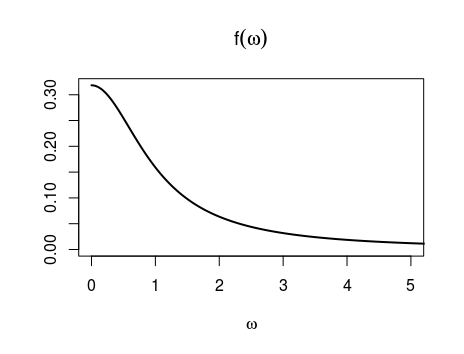
\includegraphics[width=0.48\textwidth]{dens_ex.png}
	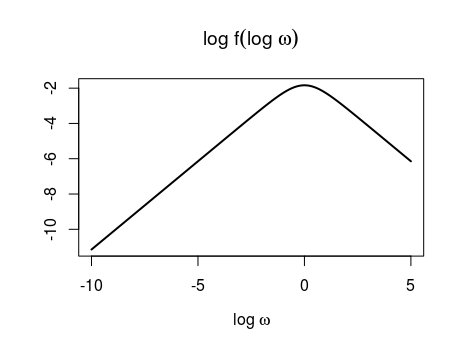
\includegraphics[width=0.48\textwidth]{logdens_ex.png}
	\caption{\small A density $f(\omega)$ with power law tails (left) and the same density transformed to the log-log scale (right). Both the left and right tails of the transformed density are linear.}
	\label{fig:logdens_ex}
\end{figure}

An important benefit to working in this log-transformed space is that linear tails are ideal for modeling the curve using a natural spline basis, which is constructed to ensure linearity beyond the outermost (\emph{boundary}) knots. If we are willing to assume that the tails of $\log f(\log \omega)$ are truly linear, then fitting it with natural splines will result in a good approximation over then entire domain $\log \omega \in (-\infty, \infty)$ without needing to use a large number of basis functions.

It might appear that requiring that $f(\omega)$ have power law tails is more restrictive than we would like. After all, the goal is to avoid the need to restrict $C(h)$ to a particular parametric family. However, the class of covariance functions that result from the Fourier transform of power law spectral densities is significantly broader than any of the parametric families, yet Bochner's theorem still guarantees that they are positive definite. In fact, this class covers most covariance models of practical interest, include the entire Mat\'ern class with finite $\nu$. Gaussian processes with spectral densities that decay quickly, e.g. with exponential tails, yield realizations that are generally regarded as unrealistically smooth~\cite{Stein1999}. %Two spatial locations a moderate distance apart would have nearly zero covariance, which is not an acceptably accurate model for real spatial data. By exclusively working with spectral densities that decay more slowly, we are restricting ourselves to the more realistic scenario where two locations can be far apart but still have a non-negligible covariance between them.

To model $\log f(\log \omega)$ using natural cubic splines, let
\begin{equation} \label{eq:spline}
	\log f(\log \omega) = \sum_{k=1}^K \beta_k B_k(\log \omega),
\end{equation}
where $\bm{\beta} = (\beta_1, \dots, \beta_K)^T$ are coefficients associated with $K$ known cubic spline basis functions $B_1(\cdot), \dots, B_K(\cdot)$. The $K$ basis functions are centered around a collection of $K$ locations referred to as knots.

% section semiparametric_modeling_of_the_spectral_density (end)

% section calculating_the_likelihood (end)

\section{Estimating the Spline Coefficients} % (fold)
\label{sec:estimating_the_spline_coefficients}


For a given collection of basis functions, the likelihood of the parameter vector $\bm{\theta} = \bm{\beta} = (\beta_1, \dots, \beta_K)^T$ can be approximated by plugging \eqref{eq:cov-elements-spectral} into \eqref{eq:loglik}. To be explicit, in \eqref{eq:loglik} the estimated covariance matrix $\bm{\Sigma}$ is expressed as a function of $\bm{\beta}$ because
\[
	\Sigma_{ij} = \int \cos(h_{ij}\omega) \, f_{\bm{\beta}}(\omega) \, d\omega \approx  \frac{1}{M} \sum_{m=1}^M \cos(h_{ij} \widetilde{\omega}_m) = \widehat{\Sigma}_{ij},
\]
\[
	\widetilde{\omega}_m \overset{\textrm{i.i.d.}}{\sim} f_{\bm{\beta}}(\omega),
\]
and
\[
	\log f_{\bm{\beta}}(\log \omega) = \sum_{k=1}^K \beta_k B_k(\log \omega).
\]
The only free parameters in this procedure are the elements of $\bm{\beta}$. This is summarized in Algorithm~\ref{alg:lik}.

To quickly generate the samples $\widetilde{\omega}_1, \ldots, \widetilde{\omega}_M$, we transform $\log f_{\bm{\beta}}(\log \omega)$ back to $f_{\bm{\beta}}(\omega)$, integrate numerically, and sample via the inverse CDF method.

\begin{algorithm}[!htb]
	\caption{\small Calculating the log likelihood $\hat{\ell}(\bm{\beta}; \bm{y})$} \label{alg:lik}
	\begin{algorithmic}[1]
		\Procedure{Likelihood}{$\bm{\beta}, \bm{y}$}
		\State $\log f_{\bm{\beta}}(\log \omega) = \sum_{k=1}^K \beta_k B_k(\log \omega)$\Comment{$k$ preselected knot locations}
		\State Sample $\widetilde{\omega}_1, \dots, \widetilde{\omega}_M$ from $f_{\bm{\beta}}(\omega)$\Comment{Inverse CDF method; $M$ large}
		\For{$1 \leq i,j \leq n$}
			\State $\widehat{\Sigma}_{ij} = \frac{1}{M} \sum_{m=1}^M \cos(h_{ij} \widetilde{\omega}_m)$\Comment{$h_{ij}$: distance between locations $\bm{s}_i$ and $\bm{s}_j$}
		\EndFor
		\State $\hat{\ell}(\bm{\beta}; \bm{y}) = -\frac{n}{2} \log(2\pi) - \frac{1}{2} \log |\widehat{\bm{\Sigma}}| - \frac{1}{2} \bm{y}^T \widehat{\bm{\Sigma}}^{-1} \bm{y}$
		\EndProcedure
	\end{algorithmic}
\end{algorithm}

Since we can calculate the likelihood as a function of the data and $\bm{\beta}$, we can estimate $\bm{\beta}$ using a Markov chain Monte Carlo (MCMC) algorithm. %However, the problem of choosing how many knots to use and where they should be located still remains.

To complete the model, we specify priors for $\bm{\beta}$ according to the Bayesian formulation of penalized splines introduced in~\cite{lang2004bayesian}.  The penalization corresponds to priors that specify to a second-order random walk, with
\[
	\beta_k \;|\; \tau^2 \sim \mathcal{N}(2\beta_{k-1} - \beta_{k-2}, \; \tau^2)
\]
where
\[
	\beta_2 \;|\; \tau^2 \sim \mathcal{N}(\beta_1, \; \tau^2)
\]
and
\[
	\beta_1 \;|\; \tau^2 \sim \mathcal{N}(0, \; \tau^2).
\]
The variance parameter $\tau^2$ controls the smoothness of the spline fit, and must also be estimated. Its prior is specified as
\[
	\tau^2 \sim \mathcal{N}^+(0, \; \sigma^2_\tau),
\]
the half-normal distribution with some variance hyperparameter $\sigma^2_\tau$.

With the priors specified, we can proceed with the MCMC algorithm in Algorithm~\ref{alg:mcmc}. We use a Metropolis-Hastings update to determine whether or not to accept the joint proposal $\bm{\beta}$. The result is random draws from the posterior distribution of $\bm{\beta} \;|\; \bm{y}$.

\begin{algorithm}[!htb]
	\caption{\small Metropolis-Hastings Sampler} \label{alg:mcmc}
	\begin{algorithmic}[1]
		\Procedure{MCMC}{$\bm{\beta}, \bm{y}$}
		\State $\bm{\beta}_1 \gets \bm{\beta}$\Comment{Initialization}
		\For{$2 \leq i \leq N$}\Comment{$N$ large}
		\State Propose new $\bm{\beta}^* \sim q(\cdot)$
		\State $\ell_0 = \hat{\ell}(\bm{\beta}_{i-1}, \bm{y})$\Comment{See Algorithm~\ref{alg:lik}}
		\State $\ell_1 = \hat{\ell}(\bm{\beta}^*, \bm{y})$
		\State $a = \Big[\pi(\bm{\beta}^*) \cdot \ell_1 \cdot q(\bm{\beta}_{i-1}|\bm{\beta}^*)\Big]/\Big[\pi(\bm{\beta}_{i-1}) \cdot \ell_0 \cdot q(\bm{\beta}^*|\bm{\beta}_{i-1})\Big]$
		\State Generate $u \sim Unif(0, 1)$
		\If{$u < \min(a, 1)$}
		\State $\bm{\beta}_i \gets \bm{\beta}^*$\Comment{Accept the proposal}
		\Else
		\State $\bm{\beta}_i \gets \bm{\beta}_{i-1}$\Comment{Reject the proposal}
		\EndIf
		\EndFor
		\EndProcedure
	\end{algorithmic}
\end{algorithm} 



% section estimating_the_spline_coefficients (end)

\section{Computational Challenges} % (fold)
\label{sec:computational_challenges}

The primary difficulty inherent in this method is that it is extraordinarily computationally intensive, requiring a Monte Carlo approximation for every element of the covariance matrix. For a moderately large number of observations, say $n = 400$, we need to estimate $\frac{n(n-1)}{2} = 79800$ separate elements. For each of these elements, we need to perform a Monte Carlo integration with a large number of samples. This all happens within one likelihood calculation, and we need to compute the likelihood at every iteration of the MCMC algorithm. The computational costs would be prohibitive for a na\"{i}ve implementation of this method.

Fortunately, most of these difficulties can be assuaged by taking advantage of parallel computing. Algorithm~\ref{alg:mcmc} requires previous information $\bm{\beta}_{i-1}$ to compute $\bm{\beta}_i$, so unfortunately it would be extremely difficult to restructure it in a way where multiple updates are being performed simultaneously. However, it is possible to parallelize aspects of the likelihood calculation in Algorithm~\ref{alg:lik}.

Consider the \textbf{for} loop in Algorithm~\ref{alg:lik}. For each value of $i$ and $j$, the computation of $\widehat{\Sigma}_{ij}$
\[
	\frac{1}{M} \sum_{m=1}^M \cos(h_{ij} \widetilde{\omega}_m)
\]
depends on two values: $h_{ij}$, the distance between $\bm{s}_i$ and $\bm{s}_j$, and $\widetilde{\bm{\omega}}$, the vector of $M$ samples from $f(\omega)$. It does not depend on any previously computed element of $\widehat{\bm{\Sigma}}$. Therefore, performance would improve dramatically if we could calculate the estimates simultaneously, in parallel.

There are several options for speeding up a parallelizable problem. The simplest, and least reliant on expensive additional hardware, is \emph{parallel processing}~\cite{suchard2010understanding}. Today, most personal computers ship with CPUs that contain 2, 4, or even 8 computing cores. Each core is capable of running a single set of sequential instructions. By using tools such as OpenMP, users can write code that will assign a set of instructions to every available core. The instructions will execute simultaneously, and the results are gathered together upon completion. Of course, the potential speedup is limited by the number of cores available in the CPU---if there are 4 cores, the instructions will be executed in about one fourth of the time.

This type of parallel processing works well for problems like obtaining multiple MCMC chains at the same time. For the estimation of $\bm{\Sigma}$ in this context, however, it is not optimal. Recall that for $n = 400$, we need to estimate $79800$ elements of $\bm{\Sigma}$. Reducing this by a factor of 4 is helpful, but ideally we would like to perform all $79800$ at once, not just take them four at a time.

Another option is to utilize a computing cluster. Clusters usually are large rooms filled with racks of computers, connected in such a way that one process can be spread uniformly across them and use hundreds or thousands of cores at once~\cite{suchard2010understanding}. One downside to this approach is that access to such a cluster is difficult to get, outside of a large company or academic institution. Beyond that, though, latency starts to become a problem when dealing with clusters. Because the cores are spread over many physical computers, the increases in computational speed becomes overwhelmed by the large amount of time it takes to share data between the cores. As a result, the overall performance increase may not be as large as we might expect.

A third option is \emph{GPU computing}. Originally created to run video games, graphics processing units, or GPUs, have become increasingly popular for parallel computing. CPUs contain a small number of cores that are optimized to handle highly complex instructions quickly. By contrast, GPUs are made up of thousands of simple, highly efficient cores that are optimized for simpler instructions and designed to work in parallel with each other. Because the GPU cores lack many of the sophisticated features of CPU cores (a sacrifice made in exchange for speed and efficient exchange of data), the programmer must have a more intricate knowledge of the architecture of their particular GPU in order to get the best possible speedup. Fortunately, directives such as OpenACC let the compiler make most of the architecture-related decisions instead of leaving them in the hands of the user.

To take full advantage of the highly parallelizable nature of the covariance estimation problem, I have chosen the GPU option. I wrote the code to carry out the Monte Carlo integrations in CUDA C. CUDA is an API provided by Nvidia that allows users to write programs in C or Fortran that interact with Nvidia brand GPUs. Computations were done on three different hardware setups:

\begin{itemize}
	\item Nvidia GeForce GTX 1060 GPU, on a personal computer running Ubuntu 16.04;
	\item Nvidia Tesla P100 GPU, provided by Penn State University's Institute for CyberScience Advanced CyberInfrastructure (ICS-ACI);
	\item Nvidia Tesla K80 GPU, running on an Amazon EC2 instance.
\end{itemize}

With these tools, the computations can be performed fairly quickly. On the Tesla P100, one entire likelihood calculation described by Algorithm~\ref{alg:lik} with $M = 50000$ and $N = 400$ completes in just under one second.

To illustrate the power of parallel computing, and to show that this element-wise approximation to the covariance matrix is a feasible approach, Figure~\ref{fig:timings-mc} shows the results of an experiment comparing the runtime of the Monte Carlo approximation from Algorithm~\ref{alg:lik} to the runtime of the exact covariance calculation. That is, for a fixed $N$, generate 100 sets of points $\bm{s}_1, \dots, \bm{s}_N$ and their distances $h_{ij} = ||\bm{s}_i - \bm{s}_j||$. Also generate $M = 20000$ samples $\widetilde{\omega}_1, \dots, \widetilde{\omega}_M$ from the spectral density $f(\omega)$ corresponding to a Mat\`ern covariance function. Since the computational cost of the random sample generation is constant regardless of $N$, it is not included when timing.
\[
	\Sigma_{ij} = C(h_{ij})
\]
and
\[
	\widehat{\Sigma}_{ij} = \frac{1}{M}\sum_{m=1}^M \cos(h_{ij} \widetilde{\omega}_{m})
\]
100 times each, and compare the median runtimes as a function of $N$.

Notice from Figure~\ref{fig:timings-mc} that for large enough $N$, it actually becomes faster to perform a Monte Carlo approximation to the elements of $\Sigma$ than to directly plug in the distances to the covariance function $C$. In this experiment $N$ needed to be greater than about 2000, but this is of course hardware dependent.

This is not a surprising result considering the parallelized nature of the Monte Carlo approximation. As $N$ increases, the exact calculation must handle all additional computations sequentially, whereas the Monte Carlo approximation can simply allocate more cores that execute their tasks simultaneously. As a result, the Monte Carlo runtime increases more slowly with $N$ than the exact covariance runtime.

However, there are nontrivial computational costs associated with GPU computing that cause it to be significantly slower than the exact alternative when $N$ is not large. In Figure~\ref{fig:timings-mc}, it appears that the Monte Carlo runtime is more or less unchanged from $N = 40$ to $N = 400$. The bottleneck here is data transfer and allocation. For small $N$, the time required to do the calculations themselves is negligible compared to the time required to allocate memory on the GPU, transfer the spectral density samples from the CPU to the GPU, combine the results, and transfer them back to the CPU. This is the reason that sometimes, seemingly paradoxically, parallelizing a routine can cause it to execute more slowly than the equivalent sequential routine. But for large enough $N$, we expect the speedup to be substantial.

\begin{figure}[htbp]
	\centering
	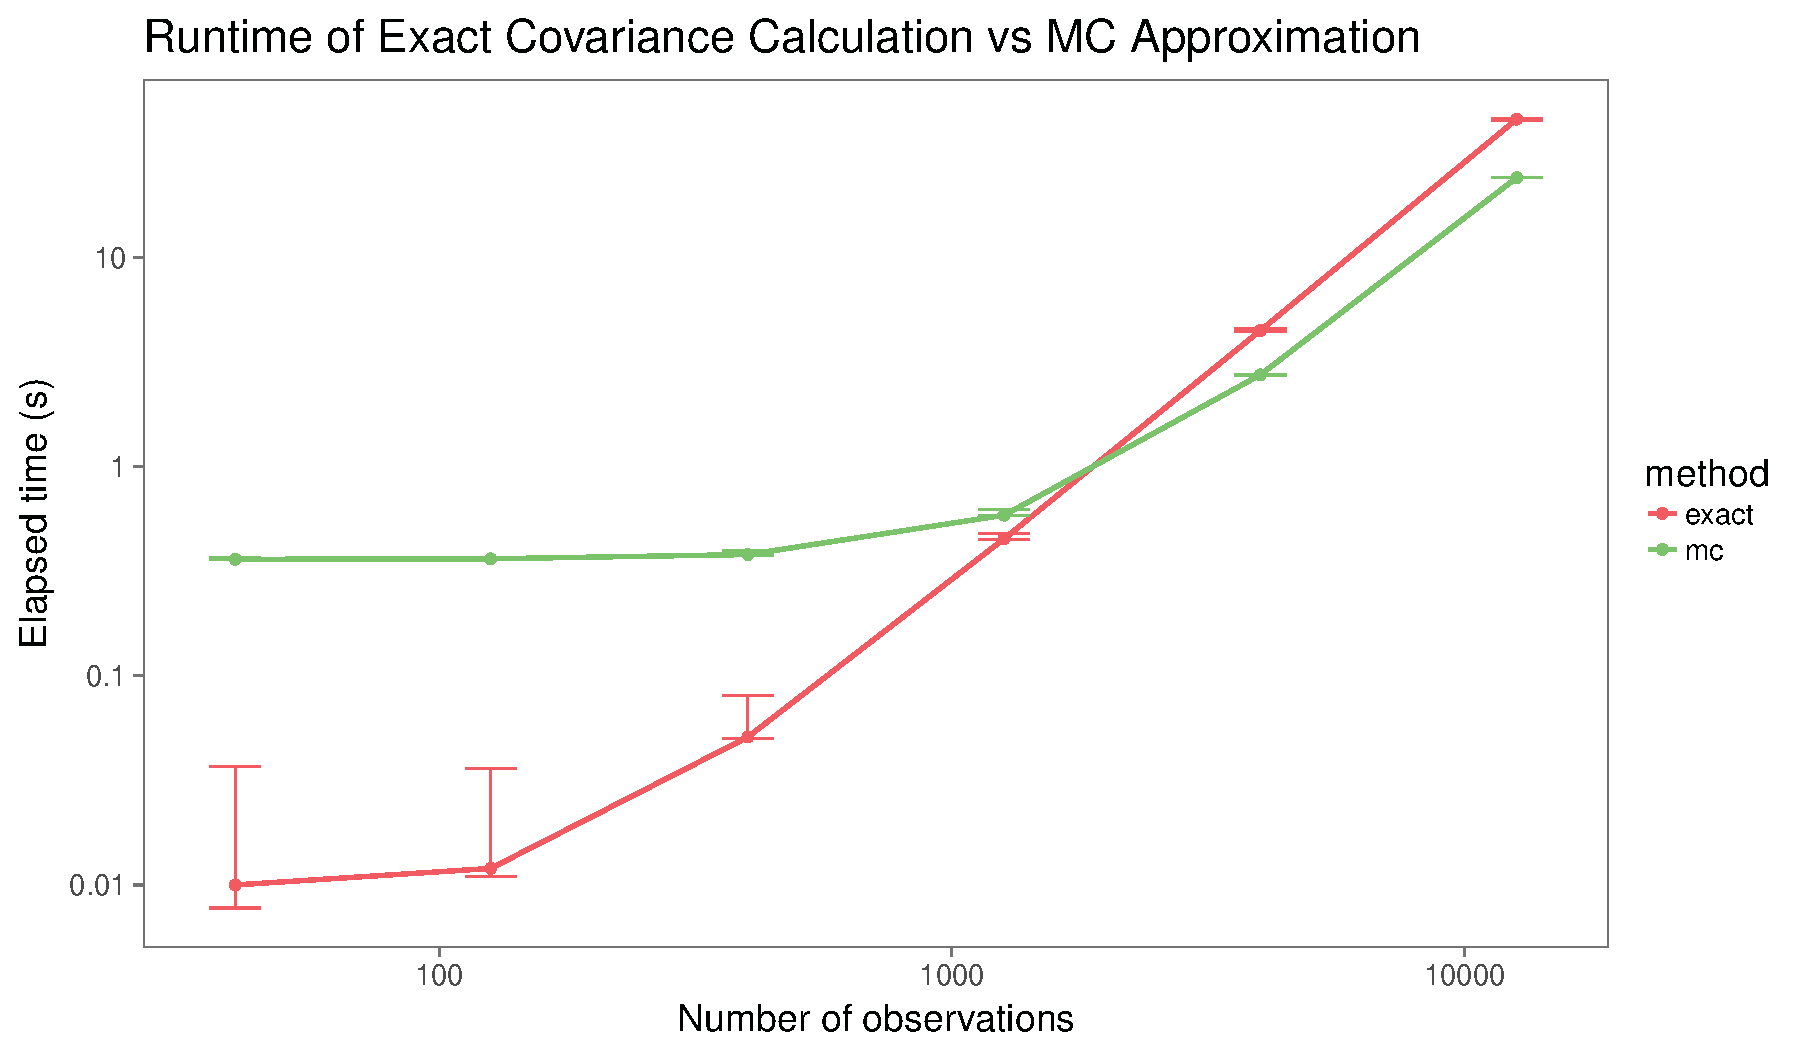
\includegraphics[width=0.95\textwidth]{timings_mc.pdf}
	\caption{Elapsed time taken to calculate the element-wise Monte Carlo approximation to the covariance matrix corresponding to a Mat\'ern covariance function, versus calculating it directly using $C(h)$. The covariance matrix is $n \times n$, where $n$ is the number of observations. Each method was run 100 times for every value of $n$. The medians are plotted with dots and connected with a line. The error bars represent the range from the first to third quartiles---some times for the exact calculation were misleadingly high due to CPU wakeup. GPU computations were done on a Tesla P100. Note the logarithmic axes.}
	\label{fig:timings-mc}
\end{figure}

% section computational_challenges (end)